\documentclass[11pt]{article}
\usepackage{common,graphicx,subfig,hyperref}

\pagenumbering{roman}
\title{CS182 Artificial Intelligence Project \\ \Large{Safety Optimised Bike Routing}}
\author{Anna Sophie Hilgard, Nick Hoernle, and Nikhila Ravi}
\begin{document}
\maketitle{}

% % Some new environments for fancy cross-referencing
% \newenvironment{a_star_algorithm}[1][htb]
%   {\renewcommand{\algorithmcfname}{$A^{*} Star Algorithm$}% Update algorithm name
%    \begin{algorithm}[#1]
%   }{\end{algorithm}}


\setlength{\parindent}{2em}
\setlength{\parskip}{1em}
\renewcommand{\baselinestretch}{1.3}
\pagenumbering{arabic}

\section{Introduction}

Biker safety and biker safety awareness have been topical issues for a number of years with the biker death toll at an unacceptably high rate (13 deaths in the past 5 years in Boston alone and 876 recorded accidents involving bikes and cars in Cambridge in the past 5 years. Current mapping applications such as Google maps often route cyclists through busy streets and intersections, resulting in unnecessary danger during trips. The purpose of this project has been to explore AI graph search and local search algorithms to optimize a bike routing algorithm not only for `distance minimization', but also for `safety' and `elevation comfort'. We explore the use of $A^{*}$ graph search under different cost and heuristic metrics to obtain a fast, yet reliable graph search between any two nodes on an intersection graph. The cost functions incorporate attributes such as distance, bike accidents and elevation, all factors which affect a cyclist's journey. Furthermore, we explore the use of local search algorithms to optimize for a central meeting point between two or more cyclists.

% \par The algorithm we chose to use for this problem is $A^{*}$ search with a variety of cost functions and heuristics incorporating distance, safety of a given route, and changes in elevation (also important for biking but not information Google maps currently considers).

% \par The graph search problem is directly analogous to techniques and ideas from the class: using intersections as nodes in the graph and road segments connecting intersections as paths, we are able to construct the city maps as directed graphs. From there, we can use data generated from a variety of sources to come up with approximate costs associated with paths and related heuristics at nodes.

% \par The optimization techniques we use are also direct applications of algorithms from the optimization portion of the course.

% Problem-specific adaptations were largely limited to the collection and interpretation of relevant data and the development of a cost function and relevant heuristics.

\section{Background and Related Work}

While the problem we were trying to solve was fairly straightforward, we conducted some preliminary research to determine potential cost parameters and data sources. Previous studies in London had explored the use of bike accident data to optimise routes for safety, and this formed the starting point for our project. Our initial formulation did not include elevation differencing, but in subsequent research, we found studies which suggested that elevation is a key factor affecting riding comfort for cyclists, and elevation data was later incorporated into our cost functions.   \cite{pmbr}.

\section{Problem Specification}
The map of a city represented as a graph of nodes (intersections) and edges (road segments) forms a highly connected state space (Cambridge has 1831 nodes, San Francisco has 18410 nodes, and each node typically has a branching factor of 4). Searching for a route through the entire state space for San Francisco, while possible, would involve considerable computational expense. There are on the order of $4^{18410}$ possible routes to explore, and this search space grows exponentially with additional nodes.
\par To extend the search problem, we tackled the task of determining central meeting areas for two or more cyclists. This search problem involves not only determining the best route from a start node to a goal, but actually determining what the best goal node is while optimizing for minimal cost for all cyclists.
\par Initially, we implemented an $A^{*}$ search algorithm for finding the optimal route between two specific notes. We used this $A^{*}$ search algorithm as a baseline, running a local search algorithm on top to find the best meeting location between two or more cyclists. We devised three cost functions and three heuristics to use with $A^{*}$ and Local Search (which depend on the $A^{*}$ algorithm), and compared the performance of each.

\section{Approach}
\subsection{Data Structures}
Our primary data structures are an intersection graph and a connection dictionary which are both stored as Python dictionaries. The intersection graph maps nodes (intersections) by a unique id to a list of paths (road segments) from that node. The connection dictionary maps a connection (road segment) to its source node, target node, and various cost parameters (distance, number of bicycle crashes on that road segment, and change in elevation over that road segment).

\subsection{Data Collection, Extraction and Preprocessing}
We were able to use open source geolocation data from Cambridge and San Francisco city councils. We were also able to obtain data on the number of accidents for various road segments from which we extracted the number of bike related accidents. Lastly an elevation layer from the open GIS website was used to infer the elevation of certain roads and intersections.

We tested the implementation of our graph structure and search algorithms on data from the cities of Cambridge, MA and San Francisco, CA. GIS location data was available on the local government websites in the form of a pandas geojson dataframe, and was easily read into a pandas dataframe object using the geopandas library \footnote{\url{http://geopandas.org/}}.
\par
The geolocation data were used to create a set of nodes with coordinate positions, and a set of connections which define the roads and the intersections that those roads are connected to. The data from Cambridge contained routing errors where some intersections were incorrectly connected to other intersections, resulting in roads that spanned the entire graph rather than simply connecting the two nearest neighboring intersections. Our solution was to use the $geometry$ data within the Pandas geolocation dataframe and the $shapely$ \footnote{https://pypi.python.org/pypi/Shapely} graphing library to compare the actual road length to our interpolated distance for the road. If the interpolated distance was incorrect by more than a factor of 10, we made the assumption that the nodes were incorrectly tagged in the data and the connection attribute was dropped. The elevation and crash data were independently collected from the different government websites, and the intersection ids were used to map this data into the `intersection' and `connection' graphs and dictionaries.
\par The resulting connected graphs for `Cambridge' and `San Francisco' are shown in figure \ref{connected_graphs}

\begin{figure}%
    \centering
    \subfloat[San Francisco]{{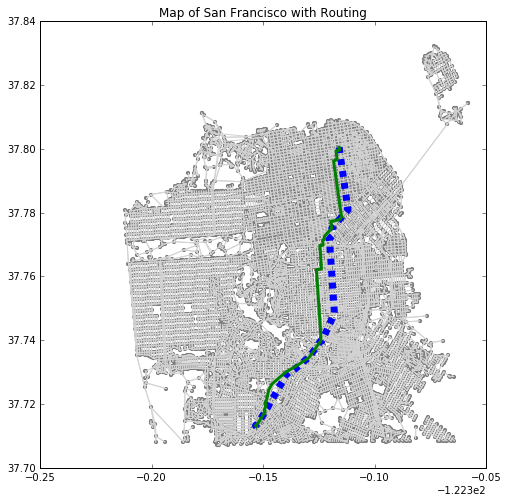
\includegraphics[width=7cm]{../images/san_fran_map} }}%
    \qquad
    \subfloat[Cambridge]{{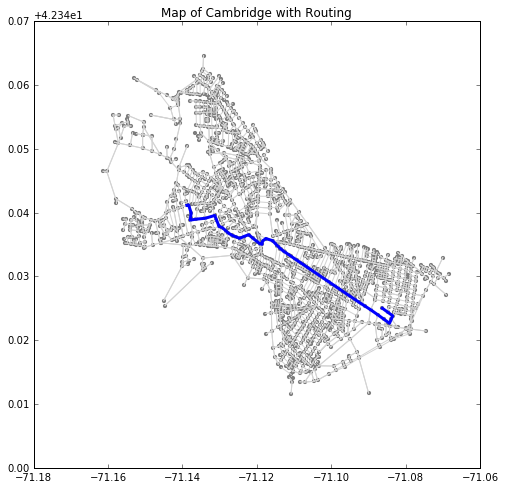
\includegraphics[width=7cm]{../images/cambridge_map} }}%
    \caption{Connected graphs of the San Francisco and Cambridge maps with a route shown on the map (using only distance as the cost metric on the Cambridge but distance and safety on the San Francisco map).}
    \label{connected_graphs}%
\end{figure}

\subsection{$A^{*}$ Search}
$A^{*}$ is an adaptive graph search algorithm that can be use to find routes based on different cost and heuristic functions passed in as parameters to the algorithm. $A^{*}$ search was chosen over the uniform cost alternative due to the possibility of a more efficient graph search under a good heuristic. Initially we started with a simple heuristic, the Euclidean distance to the goal node. We were careful to note that developing more sophisticated heuristics involving accident and elevation data is non-trivial, and may lead to inconsistent heuristic functions.\par
A formal outline of the $A^{*}$ algorithm is given in Appendix \ref{algorithms}, \nameref{a_star_algo}.

\subsubsection{Cost Functions}
The goal of $A^{*}$ search is to find a path between two nodes which minimizes some cost function:
\begin{equation}
cost = \sum_{i=0}^n cost(path_i)
\end{equation}
given that:
\begin{itemize}
\item $path_0 \in Connections_{\text{(starting node)}}$
\item $path_i, path_{i+1} \in Connections_{node_i}$
% \item $path_i, path_{i-1} \in Connections_{node_k}$
\item $path_n \in Connections_{\text{(target node - 1)}}$
\end{itemize}

\noindent Specifically for our problem, we created three different cost functions which relate to the cost attributes, distance, safety, and elevation:
\begin{align}\label{cost_fns}
cost_{distance\_only}(path_i) &= length_i \\
cost_{distance\_safety}(path_i) &= (\alpha \times length_i) \times  (\beta \times accidents_i) \\
cost_{distance\_safety\_elevation}(path_i) &= (\alpha \times length_i) \times  (\beta \times accidents_i) + abs(\Delta elevation_i)
\end{align}

\noindent  where $\alpha$ and $\beta$ are scaling multipliers to weight the relative magnitudes of the different cost measurements. We used a value of $\alpha = 10000$ to scale the coordinate based length measurement to a number on the same magnitude of $\Delta elevation$. $\beta$ was set to 5 to penalize roads with accidents by increasing their apparent length . These values can be tuned empirically.\par
\noindent In the optimization section of the project, we seek to minimize the total cost to all parties:
\begin{equation}
min(\sum_j^n cost_j)
\end{equation}
where $cost_j$ is the cost to participant j. Alternatively we could also consider minimising the difference between the maximum and minimum cost to the riders in the group. 

\subsubsection{Heuristic Functions}
We used three heuristic functions for testing the performance of the $A^{*}$ algorithm. Our baseline was a null heuristic which reduces A* to a uniform cost search. We then tried a simple admissible and consistent heuristic based on the euclidean distance from the current node to the goal node. As a more sophisticated heuristic, we created a function which is a linear combination of the estimated change in elevation from the current node to the goal, and a minimum of the number of accidents on the connections (road segments) from the current node. This `combined heuristic' also included the euclidean distance estimate. 

\begin{align}\label{heuristic_fns}
heuristic_{null}(node_i) &= 0 \\
heuristic_{euclidean\_distance}(node_i) &= euclidean\_distance(node_i, goal)\\
\begin{split}
heuristic_{combined}(node_i) &= (\alpha \times euclidean\_distance(node_i, goal) \\ &\times  (\beta \times min(accidents\_node_i)) \\&+ abs(elevation\_difference(node_i, goal))
\end{split}
\end{align}

\subsection{Local Search: Simulated Annealing}
Simulated annealing search involved initializing a centroid and iteratively hill climbing the space around the centroid to minimize the cost function in order to find a local optimum point. The temperature attribute was initialised at a high value such that the hill climbing algorithm accepts non-optimal nodes with a high probability. As the algorithm proceeds and converges on a local optimum, the temperature is decreased such that cost minimisation becomes more deterministic.
\par
As the state space of the search graph is large, and the distance metric is highly interpretable, we opted to initialize the first centroid at the intersection that represents the Euclidean mean between all cyclists. Our aim was to initialize the centroid within the vicinity of an optimal meeting point and allow the high initial temperature to counteract any potential local optimum intersections that may have been encountered.
\par
A formal outline of the algorithm is given in Appendix \ref{algorithms}, \nameref{annealing_algo}.

\subsection{Local Search: K-Beam Search}

K Beam search involved first initializing a number of centroids within the state space of the graph. The centroids were initialised in a region of the graph bounded by the starting points.  All the successors of these centroids were generated, and the k best centroids based on the cost function were chosen as the successor centroids. This iterative hill climbing from the k best centroids was used to find a local optimum. Different values of the beam width 'k', were tested to see the effect on the optimum cost and running time of the algorithm.
\par
A formal outline of the algorithm is given in Appendix \ref{algorithms}, \nameref{k_beam_algo}.

\section{Experiments}
% Analysis, evaluation, and critique of the algorithm and your
% implementation. Include a description of the testing data you used and
% a discussion of examples that illustrate major features of your
% system. Testing is a critical part of system construction, and the
% scope of your testing will be an important component in our
% evaluation. Discuss what you learned from the implementation.
We carried out a number of experiments to test the performance of our A* algorithm and various parameters. We aimed to test:
\begin{itemize}
\item The effect of the varying cost functions on the routes that were returned
\item The effect of the different $A^{*}$ heuristics on the speed of search (and consistency of the route)
\item The efficiency and effectiveness of the resulting search
\end{itemize}

\subsection{Testing $A^{*}$ Search}
We randomly selected nodes within the two graphs and ran $A^{*}$ search to find the optimal route. Figure \ref{fig:connected_san_fran} shows an example of $A^{*}$ finding an optimal route under two different costs with the safety and comfort optimised route returning a path which avoids area of high elevation. 

\begin{figure}
\center
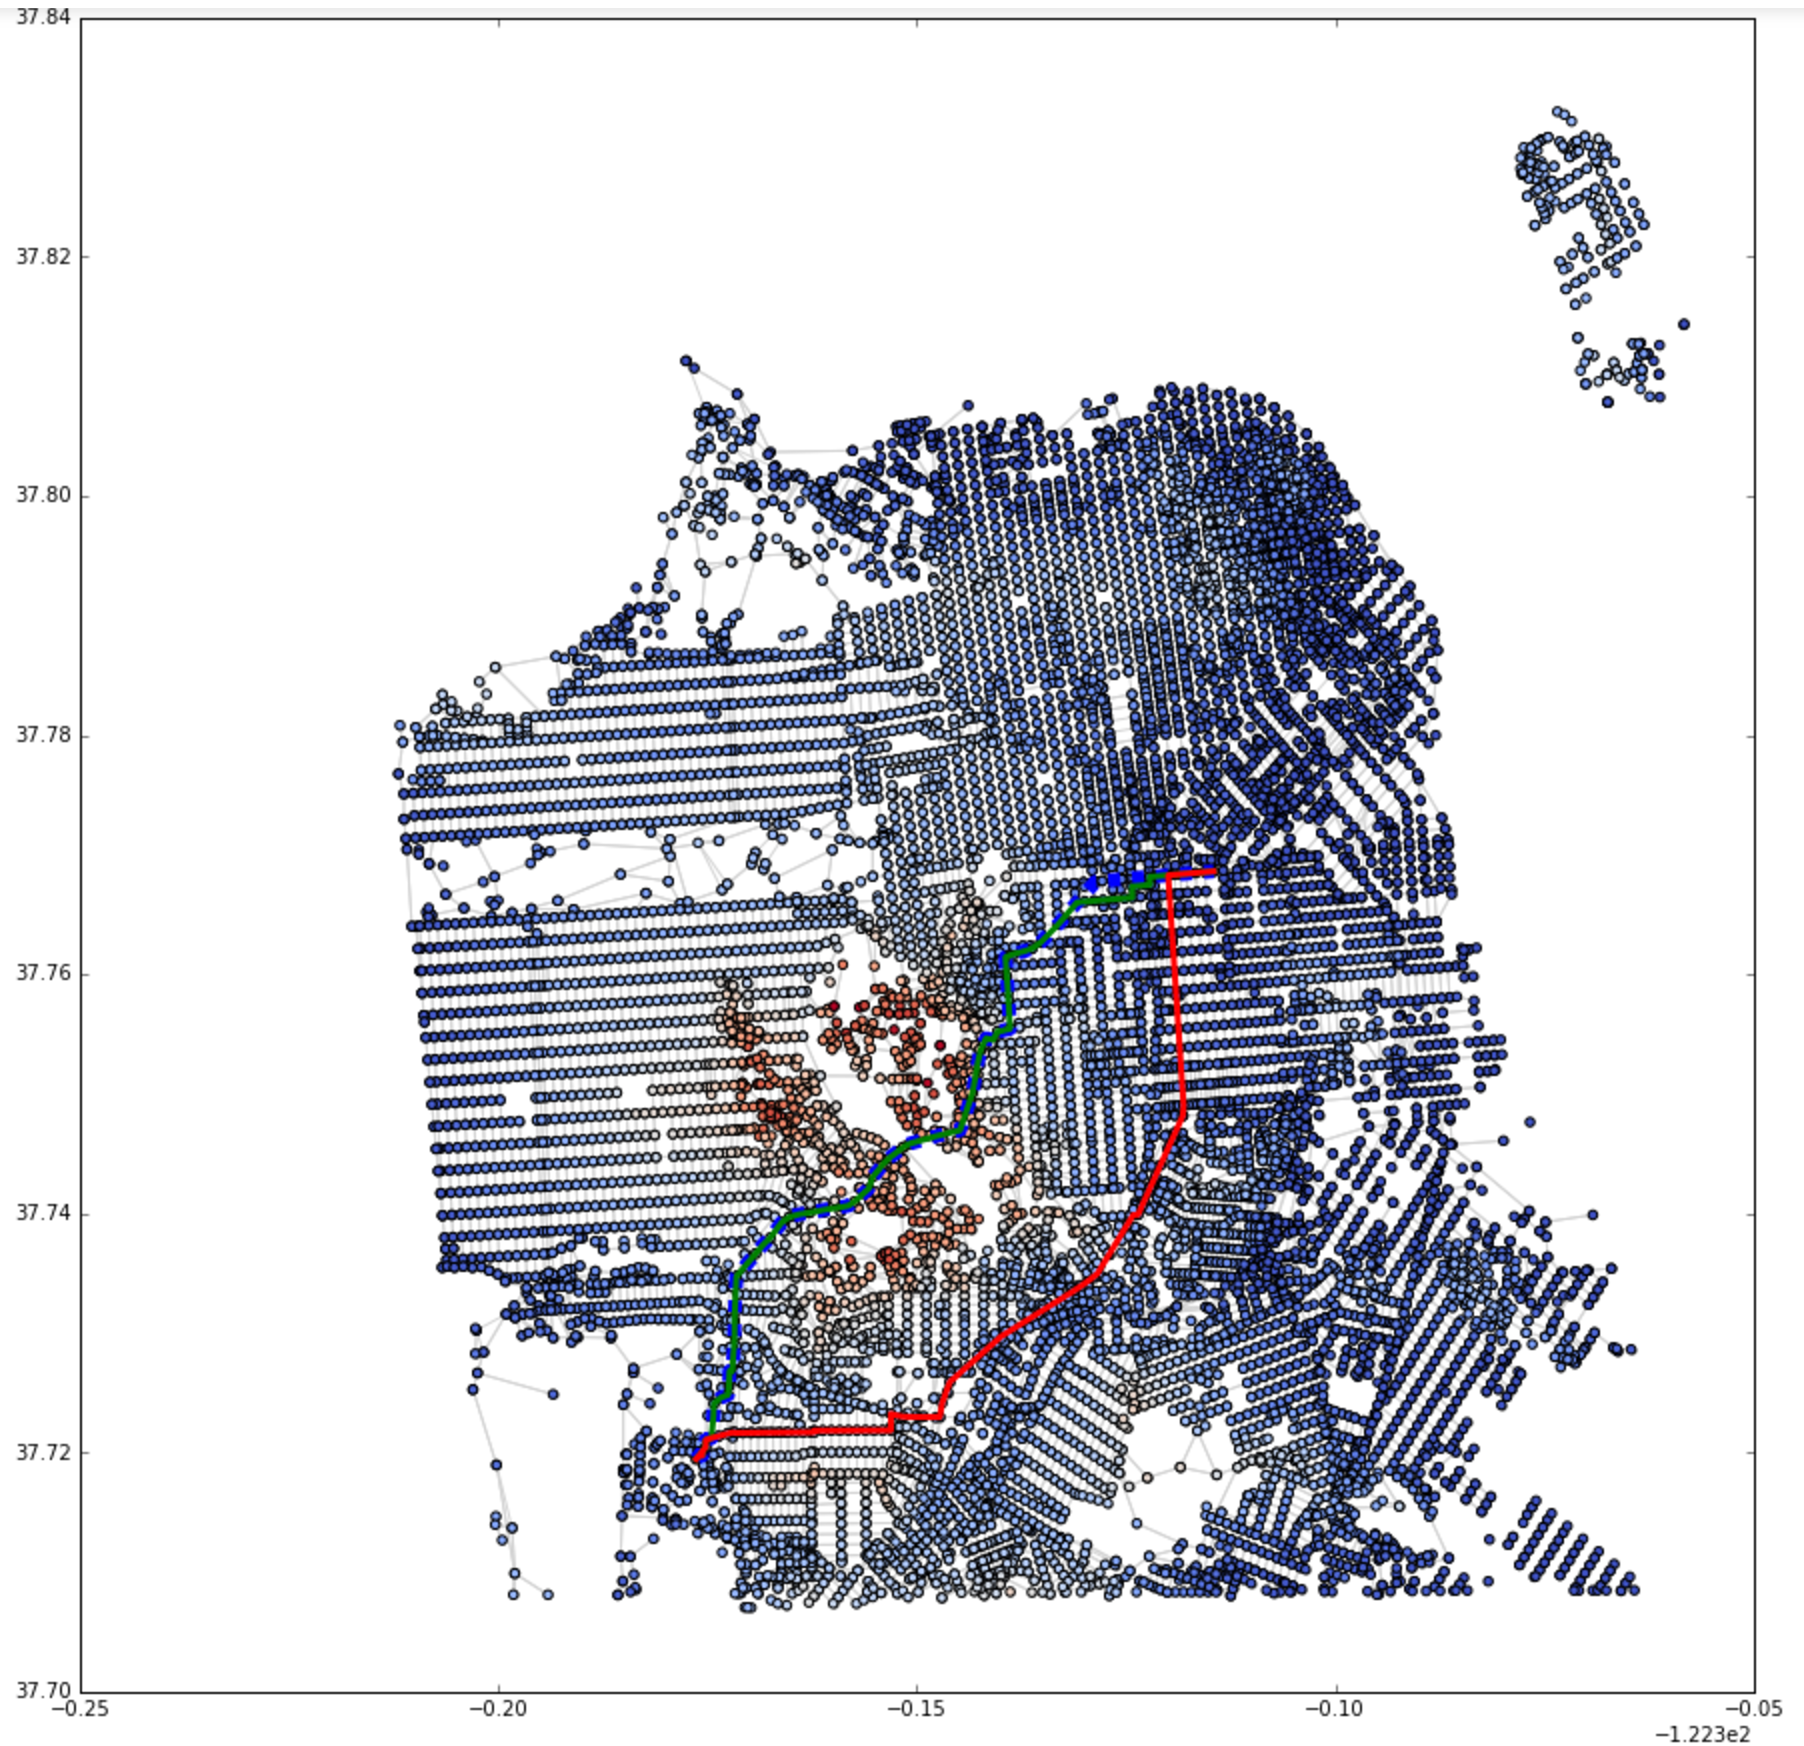
\includegraphics[width=0.6\textwidth]{../images/sf_new_plot_2.png}
\caption{Paths between nodes in San Francisco. Blue path optimizes for distance only, green path avoids previous bicycle accidents, and red path minimizes altitude changes. Overlaid with an altitude plot of San Francisco, we can clearly see the red path avoiding a hill.}
\label{fig:connected_san_fran}
\end{figure}

\par
We then ran 100 simulations for each cost function (\ref{cost_fns}) and each heuristic function (\ref{heuristic_fns}). 

We expected the null and euclidean heuristics to find the optimal route, with the euclidean heuristic exploring fewer nodes than the null heuristic. When the cost function is simple distance or simple distance and safety, the combined heuristic is neither admissible nor consistent as it is penalizing nodes for a cost that is not being used by the algorithm. With this heuristic we expect the returned optimum path to be `longer than necessary'. However, when a combined cost function is used which accounts for distance, safety and elevation, the combined heuristic is expected to out perform the other heuristics on all accounts. These results are discussed further in \nameref{results}. 

\subsection{Testing Local Search}

We ran Simulated Annealing and K-Beam Search on a number of different iterations of randomly selected nodes. While both algorithms can be tuned to run faster (by reducing the temperature faster for simulated annealing and reducing `k' for k-beam search at the cost of being more susceptible to local minima), we can make a reasonable comparison of the two algorithms in terms of their total runtime and resulting total cost of the returned centroid.

\section{Results}\label{results}

\subsection{$A^{*}$ Search Results}
Initially we ran a test of the different cost functions using a null heuristic. We are guaranteed to find the optimal solution for each of the cost functions (this is analogous to uniform cost search) even though this search is inefficient. For this experiment, we are interested in comparing the cost functions and thus efficiency was not important.
\par

Figure \ref{cost_comparison} shows the route distance, number of nodes expanded and the total change in elevation of the route for different cost functions that are used in the $A^{*}$ search. Here we see that the basic road cost will find the shortest possible route to the goal, but as additional costs are added to certain road segments, the distance of the paths returned by the other cost functions will increase. Interestingly, the three cost functions often require the same number of nodes to be searched. Lastly, we see that the combined cost function generally results in a solution that has the lowest total change in elevation (the uncommon event when it does not result in the lowest elevation is because it is also optimizing over the distance and the number of accidents on each road link).

\begin{figure}[H]
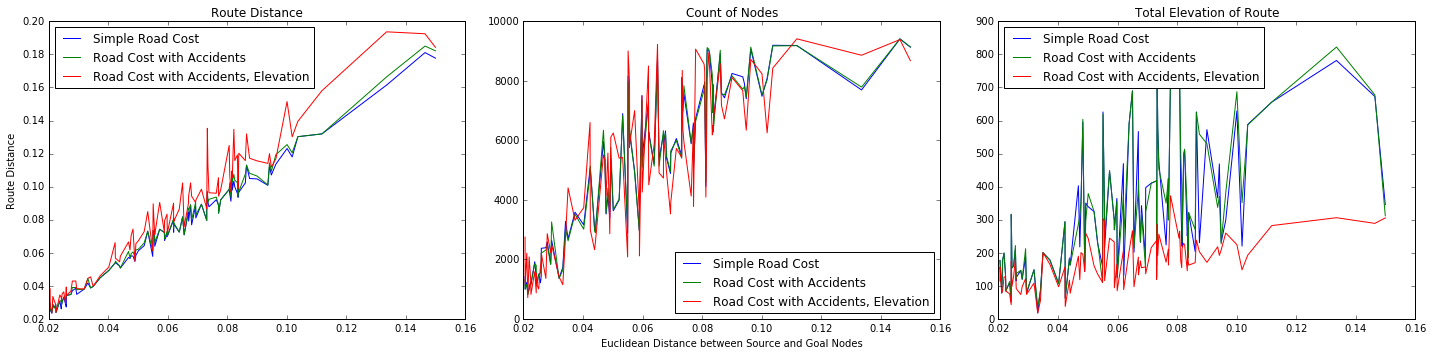
\includegraphics[width=1\textwidth]{../images/cost}
\caption{Basic metrics for the three cost functions with the null heuristic}
\label{cost_comparison}
\end{figure}

Figure \ref{simple_distance_cost} shows a comparison of the different heuristic functions under the basic road cost function. We see that the combined heuristic significantly under performs compared to the null heuristic and euclidean heuristic in terms of distance, as the combined heuristic does not properly model the cost function (it is adding expected costs for each node that are not accounted for by the basic road cost function). This heuristic is therefore not admissible for this cost function and it does not return the optimal path to the solution. The euclidean heuristic is still seen to find the optimal path and as expected, it expands far fewer nodes than the null heuristic.

\begin{figure}[H]
\caption{Varying the three heuristics for the basic road distance cost.}
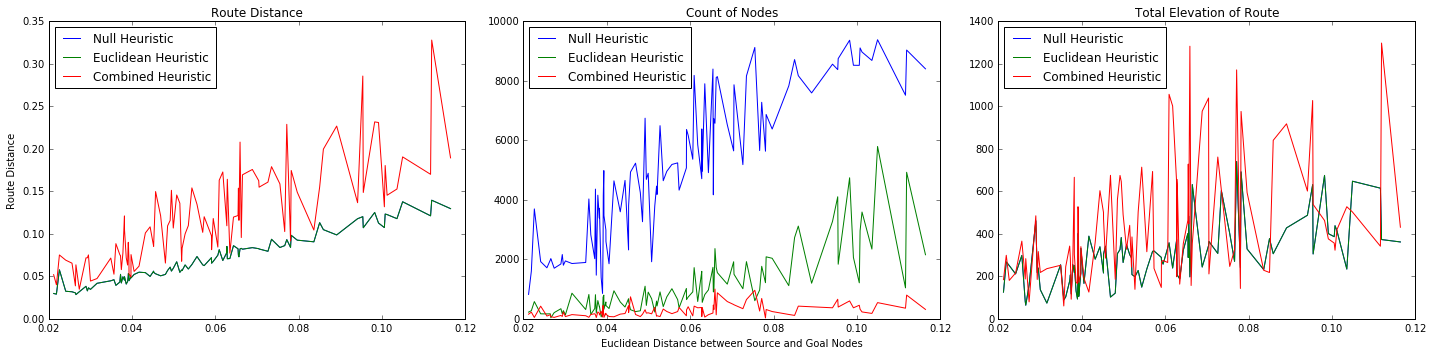
\includegraphics[width=1\textwidth]{../images/simple_distance_cost}
\label{simple_distance_cost}
\end{figure}

Figure \ref{simple_distance_and_safety} shows a similar comparison of the three heuristics now under the safety road cost (which accounts for road accidents). The results show that again, the combined heuristic is not admissible as elevation is not accounted for by the cost function. The euclidean heuristic again far outperforms the null heuristic in terms of reducing the number of nodes searched.

\begin{figure}[H]
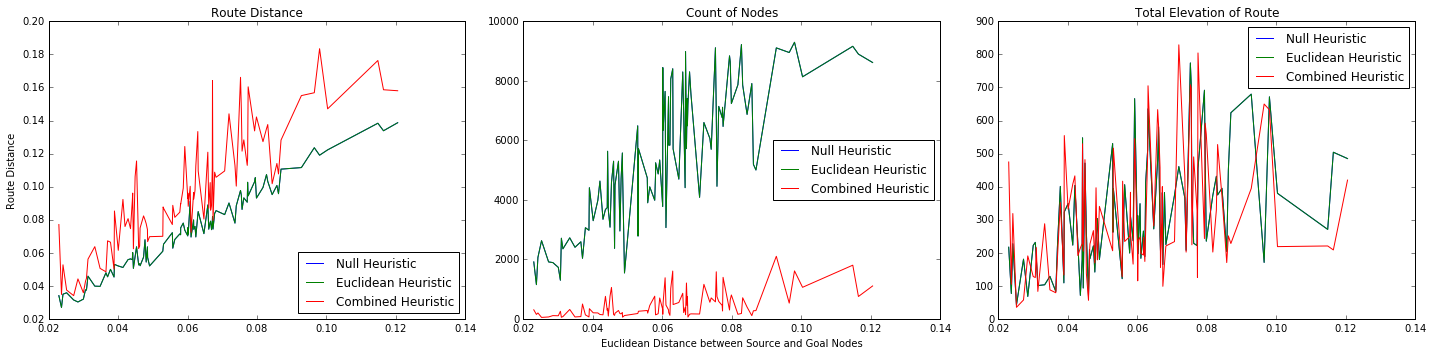
\includegraphics[width=1\textwidth]{../images/simple_distance_and_elevation}
\caption{Safety road cost under three different heuristics.}
\label{simple_distance_and_safety}
\end{figure}

Finally, \ref{simple_distance_elevation_and_safety} shows the comparison of the three heuristics under the safety road cost with elevation data also included. In this case, the the combined heuristic returns a path that is comparable to the other two heuristics (in terms of path distance). The fact the path length different suggests that the heuristic might not be admissible, as the number of accidents from one node to the next may be dramatically different from what the heuristic is guessing (this is a difficult cost parameter to model). However, the fact that this heuristic is able to model the accident and elevation costs that are calculated by the cost function means that using this heuristic is very efficient in finding an optimal route (in terms of reducing the number of nodes searched).

\begin{figure}[H]
\caption{Safety, distance, and elevation cost under three different heuristics.}
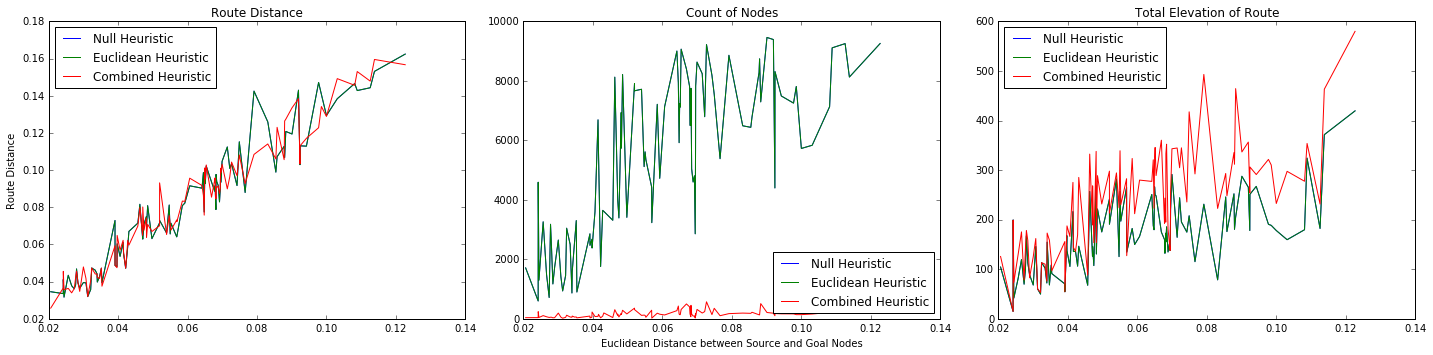
\includegraphics[width=1\textwidth]{../images/simple_distance_elevation_and_safety.png}
\label{simple_distance_elevation_and_safety}
\end{figure}

\subsection{Local Search Results}
Similar to the approach used to test the $A^{*}$ search algorithm, we randomly selected 4 nodes and computed the time that it took the algorithm to return a solution as well as the total cost. In figure \ref{sim_ann_and_k_beam_cost} we see that k beam search algorithm generally finds a solution centroid with a slightly lower cost than simulated annealing. Furthermore, from \ref{sim_ann_and_k_beam_time}, apart from under the null heuristic, we see that k beam search with $k=5$ has a very comparable search time to that of simulated annealing.

\begin{figure}[H]
\center
\caption{Time to compute the centroid node for both Simulated Annealing and K Beam search (with $k = 5$)}
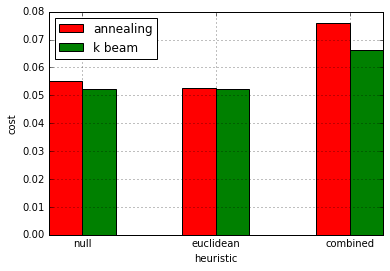
\includegraphics[width=0.6\textwidth]{../images/k_beam_sim_annealing.png}
\label{sim_ann_and_k_beam_cost}
\end{figure}

\begin{figure}[H]
\center
\caption{Total cost of routes from all starting nodes to the returned centroid for both Simulated Annealing and K Beam search (with $k = 5$)}
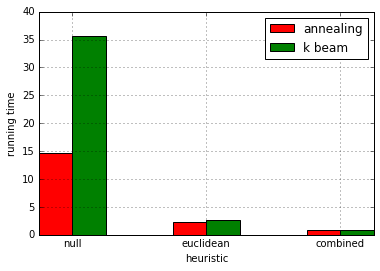
\includegraphics[width=0.6\textwidth]{../images/k_beam_sim_running_time.png}
\label{sim_ann_and_k_beam_time}
\end{figure}

The reason for k beam search out performing simulated annealing is the presence of very definite local optima. The initialization of multiple random starting points within the possible central region has a greater chance of resulting in the centroid being close to the optimal solution than with simulated annealing. Even with the temperature initialised at a high value, simulated annealing struggles to explore beyond the vicinity of the node that it is initialized at.  Since this starting node is deterministically the absolute center of all the cyclists, it may be far from the global optimum point, especially if the route is hilly or has many road accidents.
\par
While the k beam solution does outperform the simulated annealing solution, in practice we do see that the costs are still comparable and thus the solution that is returned by simulated annealing is still valid. The below figure \ref{overall_plot} is a plot showing the centroid found between four cyclists (under the combined cost function and combined heuristic).

\begin{figure}[H]
\caption{Plot showing the centroid found between four cyclists in Cambridge, and each cyclist's route to the solution. The plot encodes the cost of every other node in the map as if it were the centroid (and thus shows the high cost nodes in red - i.e. unlikely centroids) and the low cost nodes in yellow (i.e. likely centroids). We further see from this plot that while the combined cost for the four cyclists is not necessarily the same as the cost of only one cyclist, the route that the $A^{*}$ algorithm finds generally follows a path that avoids the red high cost nodes.}
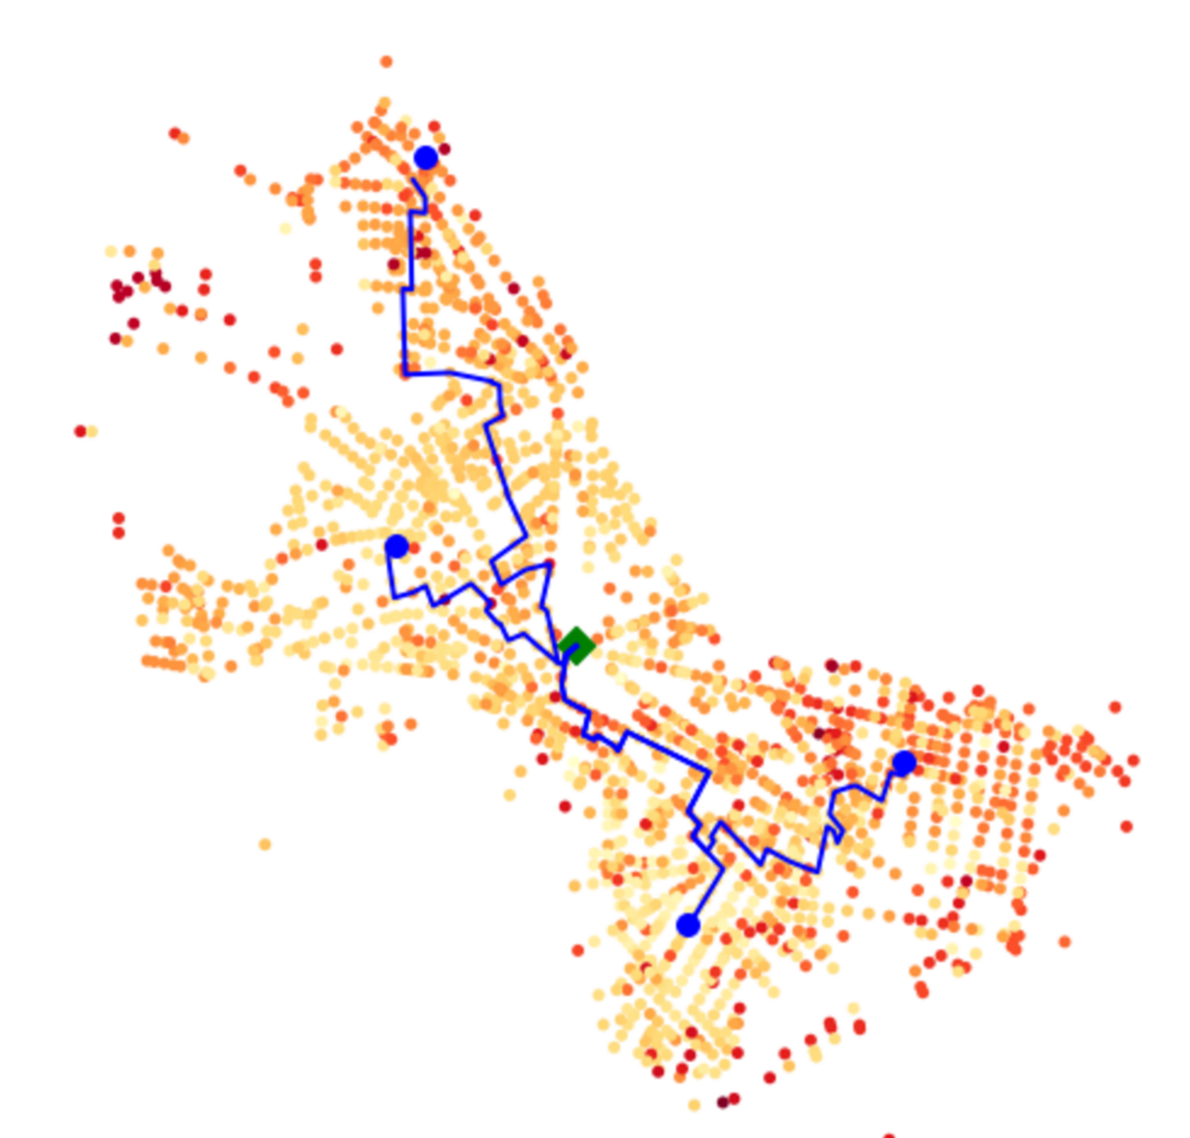
\includegraphics[width=1\textwidth]{../images/overall_plot.png}
\label{overall_plot}
\end{figure}

\section{Discussion}

Through this project we have explored a range of algorithms, cost, and heuristic functions for graph search in cities, optimising for different objectives and compared their performance.  The graph search approach offers a highly adaptive solution to the problem of intelligent bike routing. Given our pre-existing knowledge of Cambridge and San Francisco city streetscape, we felt the routes obtained under the different cost functions were reasonable. 

The running time of the algorithms we have developed could have been decreased by incorporating pruning strategies, but run times were generally satisfactory (especially when evaluating the combined heuristic with the distance, safety and elevation costs). In developing heuristics, it was difficult to generate a useful non-trivial heuristic for bike crashes which was also admissible - an extremely convoluted path could almost always be found to avoid all bike accident locations. Therefore a heuristic which is always $\le$ the actual cost to the goal is often not consistent. However, even without being consistent (i.e. it was returning a solution that was slightly different from the optimal solution), the combined heuristic did provide a good route.

\par
Furthermore, while the number of accidents per road segment is a good estimate of the danger posed by a road segment, a better indicator might be accidents per units of bicycle traffic. If we were able to collect bicycle traffic data for each road segment, we could then calculate the Bayesian probability of:
\begin{equation}
P(\text{road segment $\vert$ accident}) \propto P(\text{accident $\vert$ road segment}) * P(\text{road segment})
\end{equation}In particular, we may be overpenalizing roads with a large amount of cycling traffic.
\par

\par
\noindent Takeaways from this project:
\begin{itemize}
\item You are only as good as your data - we had high expectations for the data we would be able to collect and use for this project, however even the data we ended up using was harder to collect and map than we had originally anticipated. Furthermore, while still useful for testing the implementations of our algorithms, much of the crash data was a few years old and thus to be more applicable we would want to include real time updates to the bike accident data and an expiration of old data. Cambridge and San Francisco are relatively tech-forward cities, so we can imagine this would be even more difficult in most other cities.
\item We initially built the system for the Cambridge data but then obtained the larger dataset for San Francisco. It was therefore interesting to see how our algorithms scaled to the larger map. To plan routes through a larger graph, it is clear that we would have to adapt the algorithm to improve the runtime performance to be within a reasonable range. Our background research suggested that many routing engines actually use inadmissible heuristics to reduce the running time but are still able to find reasonable results. 
\end{itemize}

\begin{thebibliography}{9}
\bibitem{pmbr} 
Hrncir, Jan and Zilecky, Palov and Song, Qing and Jakob, Michal
\textit{Practical Multicriteria Urban Bicycle Routing}
IEEE Transactions on Intelligent Transportation Systems, PP 99 2016, pg 1-12
\bibitem{routing} 
Alex D. Singleton and Daniel J. Lewis
\textit{Including Accident Information in Automatic Bicycle Route Planning for Urban Areas}
Urban Studies Research Volume 2011, Article ID 362817
\bibitem{routeplanning} 
Botea, Nikolova, Berlingerio
\textit{Multi-Modal Journey Planning in the Presence of Uncertainty}
Twenty-Third International Conference on Automated Planning and Scheduling
\bibitem{routes} 
Daniel Delling, Andrew V. Goldberg,Thomas Pajor, and Renato F. Werneck
\textit{Customizable Route Planning}
Microsoft Research
\end{thebibliography}

\section*{Data Sources}
\begin{itemize}
\item City of Cambridge GIS data GEOJSON files \\
\texttt{ http://cambridgegis.github.io/gisdata.html}
\item Accidents - list of crashes involving motor vehicles, bicycles and/or pedestrians reported in the City of Cambridge from January 2010 through June 2016 \\
\texttt {https://data.cambridgema.gov/Public-Safety/Crashes/ybny-g9cv/data} \\
\end{itemize}


\newpage
\appendix
\section{System Description}

The easiest way to use our system is to clone the \href{https://github.com/NickHoernle/Artificial-Intelligence-CS182-Project/blob/master/}{Github Repo} where the code is hosted, open the provided iPython notebook, and run each of the cells. All of the supporting functions can be found in $final\_project.py$.\footnote{$final\_project.py$: \url{https://github.com/NickHoernle/Artificial-Intelligence-CS182-Project/blob/master/final_project.py}} \footnote{$final\_project.ipynb$: \url{https://github.com/NickHoernle/Artificial-Intelligence-CS182-Project/blob/master/final_project.ipynb}}

\section{Group Makeup}

\begin{enumerate}
\item Nicholas Hoernle
\begin{enumerate}
\item Creation of graph dictionary structure and $A^{*}$search algorithm
\item Simulated annealing
\end{enumerate}
\item Nikhila Ravi
\begin{enumerate}
\item K-Beam Search
\item Visualization and analysis of results of graph search algorithms
\end{enumerate}
\item Anna Sophie Hilgard
\begin{enumerate}
\item Construction of Datasets
\item Research and Implementation of more complicated cost functions and heuristics
\end{enumerate}
\end{enumerate}

\section{Algorithms}\label{algorithms}
\begin{algorithm}[H]
  \caption{$A^{*}$ Search Algorithm}\label{a_star_algo}
  \begin{algorithmic}
    \Function{A-Star-Search}{$graph, start node, target node$}
    \State{$node \gets $a node with $ \textsc{state}=start node$}
    \State{$\textsc{path-cost} \gets \textbf{heuristic}(start node, target node)$}
    \State{$frontier\gets $ a priority queue ordered by $\textsc{path-cost} + \textbf{heuristic}(node, target node)$ with $node$ as the only element}
    \State{$explored \gets $ an empty set}
    \Loop
    \If{$\textsc{Empty?}(frontier)$}
    \State \textbf{return failure}
    \EndIf
    \State{$node \gets \textsc{pop}(frontier)$ /*chooses the lowest cost+heuristic node in $frontier$ */}
     \If{$node == targetnode$}
    \State {\textbf{return} \textsc{solution}($node$)}
    \EndIf
    \State{add node.\textsc{State} to $explored$}
    \For{ \textbf{each} $path$ in \textsc{Paths}($node$)}
    \State{$child \gets$ \textbf{child-node}($node, path$)}
    \If {$child$.\textsc{State} is not in $explored$ or $frontier$}
    \State{$frontier \gets$ \textbf{insert}($child, frontier$)}
    \ElsIf  {$child$.\textsc{State} is in $frontier$ with higher \textsc{path-cost} + heuristic}
    \State{replace that $frontier$ node with $child$}
    \EndIf
    \EndFor
    \EndLoop
    \EndFunction{}
  \end{algorithmic}
  \caption{A-Star Search}
\end{algorithm}

\begin{algorithm}[H]
  \caption{Simulated Annealing Algorithm}\label{annealing_algo}
  \begin{algorithmic}
    \Function{Simulated Annealing Meeting Spot}{$graph, startingpts, cost, heuristic$}
    \If{$\textbf{length}(startingpts)<2$}
    \State \textbf{return error}
    \EndIf
    \State{$current \gets$ \textbf{mean}$(startingpts)$.\textsc{closest-node}}
    \State{$temperature \gets e^{10}$}
    \State{$\gamma \gets .5$ /*schedule to manage $temperature$ */}
    \While{$temperature > e^{-2}$}
      \State{$temperature \gets temperature*\gamma$}
      \State{$next \gets$ a randomly selected $child$ of $current$}
      \State{$current.\textsc{value} \gets \sum_{pt \in startingpts}\textbf{cost}(pt, centroid$)}
      \State{$next.\textsc{value} \gets \sum_{pt \in startingpts}\textbf{cost}(pt, next$)}
      \State{$\Delta E \gets next.\textsc{value} - current.\textsc{value}$}
      \If {$\Delta E > 0$}
      \State{$current \gets next$}
      \Else
       \State{$current \gets next$ with probability $e^{\Delta E / temperature}$}
      \EndIf
    \EndWhile
    \EndFunction{}
  \end{algorithmic}
\end{algorithm}

\begin{algorithm}[H]
  \caption{K Beam Search Algorithm}\label{k_beam_algo}
  \begin{algorithmic}
    \Function{K-Beam Search Meeting Spot}{$k, graph, startingpts, cost, heuristic$}
    \If{$\textbf{length}(startingpts)<2$}
    \State \textbf{return error}
    \EndIf \\
    \State{$\{candidatenodes\} \gets \,node\, \forall \,node \in graph $ s.t. \\ $node.x \ge min(startingpts.x) \& \,node.x \le max(startingpts.x) \&$ \\ $node.y \ge min(startingpts.y) \& \,node.y \le max(startingpts.y)$} \\
    \State{$point_i \gets$ a randomly selected $node \in \{candidatenodes\} \forall i \le k$}
    \State{$best.\textsc{value} \gets min_{i\le k}(\sum_{pt \in startingpts}\textbf{cost}(pt, point_i))$}
    \While{\textbf{True}}
      \State{$\{nextcosts \} \gets \sum_{pt \in startingpts}\textbf{cost}(pt, child_i) \forall i \le k, child_i \in \textsc{Paths}(point_i).endnode $}
      \State{$point_i \gets$ i-th least $node \in \{nextcosts\} \forall i \le k$}
      \State{$next.\textsc{value} \gets \sum_{pt \in startingpts}\textbf{cost}(pt, point_1$)}
      \If {$next.\textsc{value} < best.\textsc{value}$}
      \State{$best \gets next$}
      \Else
       \State{\textbf{break}}
      \EndIf
      \State{\textbf{return} $best$}
    \EndWhile
    \EndFunction{}
  \end{algorithmic}
\end{algorithm}

\bibliographystyle{plain} 
\bibliography{project-template}

\end{document}
